\documentclass{article}
\usepackage[utf8]{inputenc}
\usepackage{polski}
\usepackage{geometry}
\usepackage{pdfpages}
\usepackage{pdfpages}
\usepackage{listings}
\usepackage{listingsutf8}
\usepackage{multirow}
\usepackage{siunitx}
\usepackage{multirow}
\usepackage{booktabs}
\usepackage{tabularx}
\usepackage{placeins}
\usepackage{pdflscape}
\usepackage{graphicx}
\usepackage{subfig}
\usepackage{hyperref}
\usepackage{amsmath}
\usepackage{colortbl}

\geometry{
a4paper,
total={170mm,257mm},
left=20mm,
top=20mm
}
\newcolumntype{Y}{>{\centering\arraybackslash}X}
% \renewcommand\thesection{}
\lstset{%
literate=%
 {ą}{{\k{a}}}1
 {ę}{{\k{e}}}1
 {Ą}{{\k{A}}}1
 {Ę}{{\k{E}}}1
 {ś}{{\'{s}}}1
 {Ś}{{\'{S}}}1
 {ź}{{\'{z}}}1
 {Ź}{{\'{Z}}}1
 {ń}{{\'{n}}}1
 {Ń}{{\'{N}}}1
 {ć}{{\'{c}}}1
 {Ć}{{\'{C}}}1
 {ó}{{\'{o}}}1
 {Ó}{{\'{O}}}1
 {ż}{{\.{z}}}1
 {Ż}{{\.{Z}}}1
 {ł}{{\l{}}}1
 {Ł}{{\l{}}}1
}

\title{Metody Programowania Równoległego\\ Cuda - Laboratorium III}
\author{Maciej Trątnowiecki}
\date{AGH, Semestr Letni, 2022}

\begin{document}
    \maketitle
    \lstset{ 
      backgroundcolor=\color{white},   % choose the background color; you must add \usepackage{color} or \usepackage{xcolor}; should come as last argument
      basicstyle=\footnotesize,        % the size of the fonts that are used for the code
      breakatwhitespace=false,         % sets if automatic breaks should only happen at whitespace
      breaklines=true,                 % sets automatic line breaking
      captionpos=b,                    % sets the caption-position to bottom
      commentstyle=\color{mygreen},    % comment style
      deletekeywords={...},            % if you want to delete keywords from the given language
      escapeinside={\%*}{*)},          % if you want to add LaTeX within your code
      %extendedchars=true,              % lets you use non-ASCII characters; for 8-bits encodings only, does not work with UTF-8
      firstnumber=1000,                % start line enumeration with line 1000
      frame=single,	                   % adds a frame around the code
      keepspaces=true,                 % keeps spaces in text, useful for keeping indentation of code (possibly needs columns=flexible)
      keywordstyle=\color{blue},       % keyword style
      language=Octave,                 % the language of the code
      morekeywords={*,...},            % if you want to add more keywords to the set
      numbers=left,                    % where to put the line-numbers; possible values are (none, left, right)
      numbersep=5pt,                   % how far the line-numbers are from the code
      numberstyle=\tiny\color{mygray}, % the style that is used for the line-numbers
      rulecolor=\color{black},         % if not set, the frame-color may be changed on line-breaks within not-black text (e.g. comments (green here))
      showspaces=false,                % show spaces everywhere adding particular underscores; it overrides 'showstringspaces'
      showstringspaces=false,          % underline spaces within strings only
      showtabs=false,                  % show tabs within strings adding particular underscores
      stepnumber=2,                    % the step between two line-numbers. If it's 1, each line will be numbered
      stringstyle=\color{mymauve},     % string literal style
      tabsize=2,	                   % sets default tabsize to 2 spaces
      title=\lstname                   % show the filename of files included with \lstinputlisting; also try caption instead of title
    }
    
    \section{Informacje sprzętowe}
    Wszystkie poniższe wyniki uzyskane zostały poprzez wykonanie pomiarów na komputerze wyposażonym w kartę graficzną \textit{Nvidia GTX 1060 6GB}.
    
    \section{Redukcja}
    Rozmiar wejścia: $2^{24}$. Zebrane wyniki ilustruje poniższy wykres.
        \begin{figure}[htb]
            \centering
            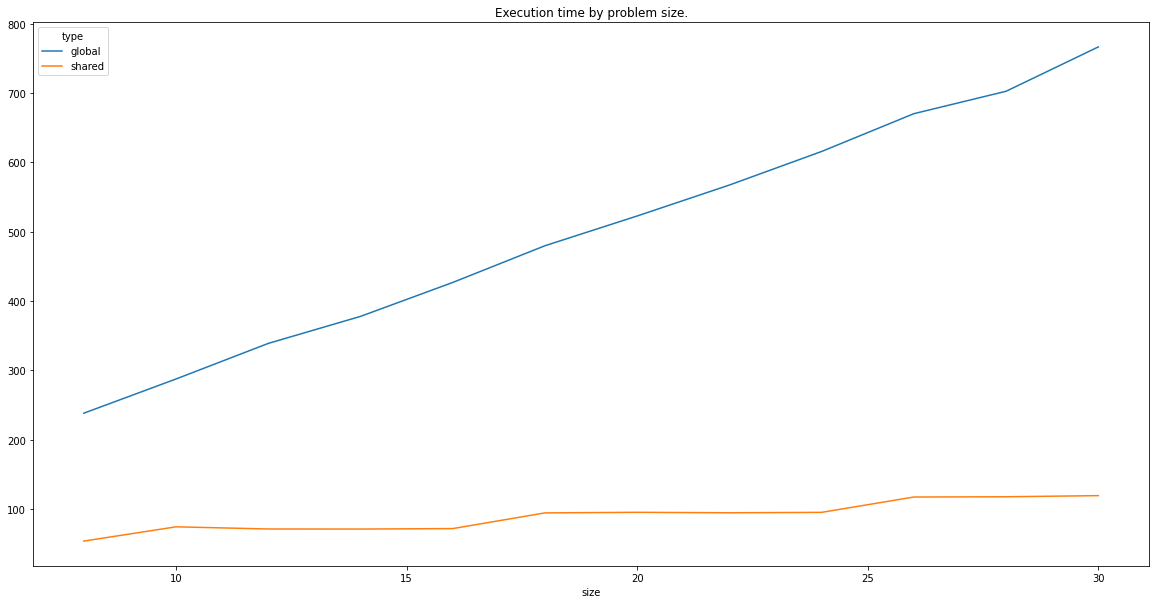
\includegraphics[width=\textwidth]{cuda/Lab3/report/images/exec_time.png}
            \caption{Czas wykonania programu w zależności od rozmiaru problemu w skali zwykłej.}
        \end{figure}
        \begin{figure}[htb]
            \centering
            
            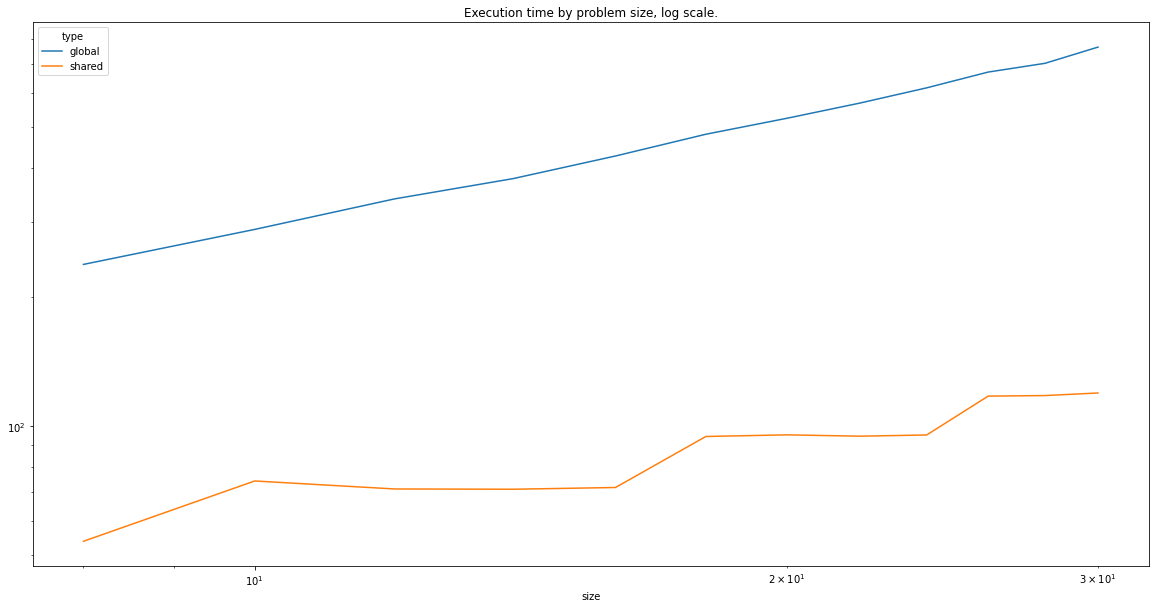
\includegraphics[width=\textwidth]{cuda/Lab3/report/images/exec_time_log.png}
            \caption{Czas wykonania programu w zależności od rozmiaru problemu w skali logarytmicznej.}
        \end{figure}
        
    \newpage
    \section{Spojrzenie na efekt „warp divergence”}
    Rozmiar wejścia: $2^{24}$. Wyniki pomiarów zebrałem w poniższej tabeli.
            \begin{center}
            % \begin{tabular}{lrrlrr}
            \begin{tabular}{|c|c|}
            \hline
             Typ & Czas wykonania \\
             \hline
            sequential & 99.011 msec \\
            interleaved & 101.595 msec\\
            \hline
            \end{tabular}
        \end{center}

    \section{Loop unrolling}
        Rozmiar wejścia: $2^{24}$. Wyniki pomiarów zebrałem w poniższej tabeli.
            \begin{center}
            % \begin{tabular}{lrrlrr}
            \begin{tabular}{|c|c|}
            \hline
             Typ & Czas wykonania \\
             \hline
            cg & 98.130 msec \\
            wp & 97.432 msec\\
            \hline
            \end{tabular}
        \end{center}

    \section{Operacje atomowe}
        Rozmiar wejścia: $2^{24}$. Wyniki pomiarów zebrałem w poniższej tabeli.
            \begin{center}
            % \begin{tabular}{lrrlrr}
            \begin{tabular}{|c|c|}
            \hline
             Typ & Czas wykonania \\
             \hline
            atomic & 48.038 msec \\
            blk & 72.145 msec\\
            wrp & 72.421\\
            \hline
            \end{tabular}
        \end{center}

    \section{Histogram}
    Rozmiar wejścia: $2000000$. Zebrane wyniki ilustruje poniższy wykres.
        \begin{figure}[htb]
            \centering
            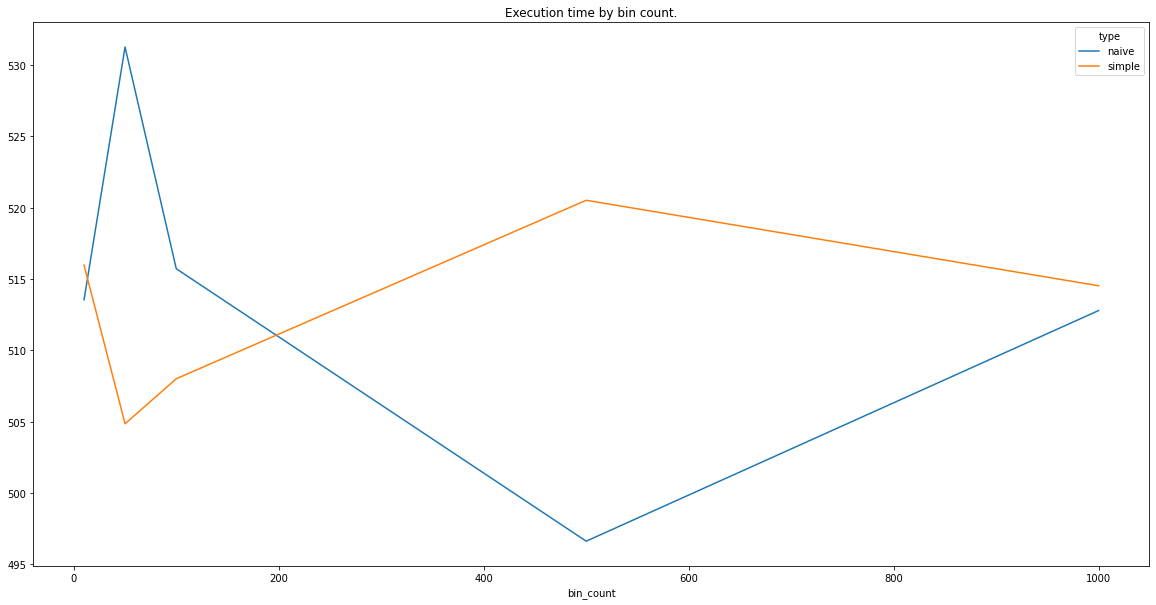
\includegraphics[width=\textwidth]{cuda/Lab3/report/images/histo.png}
            \caption{Czas wykonania programu w zależności od ilości kanałów histogramu.}
        \end{figure}
        

    \clearpage
    \section{Kod modyfikowanych programów}
        \lstinputlisting[language=c]{../5 Histogram/histo.cu}
        
\end{document}
